\documentclass[10pt,a4paper]{report}
%\usepackage[utf8]{inputenc}
\usepackage[latin1]{inputenc}
\usepackage{amsmath}
\usepackage{amsfonts}
\usepackage{amssymb}
\usepackage{multicol, blindtext}
\usepackage{textcomp}
\usepackage{graphicx}
\usepackage{lipsum}

\title{Laborat�rio de Sistemas de Controle - Relat�rio 1}

\begin{document}



%\title{Medi��o de Velocidade usando um Sensor de Luminosidade}

\author{Hugo Santos - 10080000701}
%Matr�culas: {10080000801, 10080000701, 10080000501}
%\thanks{Engenharia da Computa\c{c}\~ao, Universidade Federal do Par\'a, Bel\'em-PA, Brasil}
\maketitle

\tableofcontents


%Emails: \{dhcsouza, huggosan, weltonmaxx007\}@gmail.com\\


\chapter{Quest�o 2}

\section{Funcionamento do Script}
	O script � utilizado para fazer o c�lculo num�rico dos coeficientes da s�rie de Fourier da fun��o $\Delta(t/2)$, utilizando a f�rmula da transformada inversa mostrada na equa��o \ref{eq:formcoef} . O algoritmo do programa est� definido abaixo.

	\[ t_{p} = \dfrac{\pi}{w_{d}} \]
	
	\[ \dfrac{C(s)}{R(s)} = \dfrac{kw_{n}^{2}}{s^{2} + 2\xi w_{n} s + w^{2}_{n}} \]

	\[ \dfrac{C(s)}{R(s)} = \dfrac{K}{s^{2} + (1+KK_{h})s + K} \]

	\[ w_{d} = w_{n}\sqrt[]{1-\xi^{2}} \]
\begin{itemize}
	\item Para $w_{n}$=2, k=8 e $\xi$=1 mostrado na Figura \ref{fig:i_w2_k8_e1}
	\begin{itemize}
		\item $T_{s}$=2.893
		\item $T_{p}$ n�o foi necess�rio porque o sistema se comportou como um sistema de ordem 1
	\end{itemize}
	\item Para $w_{n}$=2, k=8 e $\xi$=0.7  mostrado na Figura \ref{fig:i_w2_k8_e07}
	\begin{itemize}
		\item $T_{s}$=2.893
		\item $V_{p}$=8.367
		\item $M_{p}$=4.5875
		\item $T_{p}$=2.157
		\item $T_{p}$=2.199 calculado
	\end{itemize}
	\item Para $w_{n}$=2, k=8 e $\xi$=0.2  mostrado na Figura \ref{fig:i_w2_k8_e02}
	\begin{itemize}
		\item $T_{s}$=9.535
		\item $V_{p}$=12.17
		\item $M_{p}$=52.12
		\item $T_{p}$=1.535
		\item $T_{p}$=1.603 calculado
	\end{itemize}
	\item Para $w_{n}$=10, k=8 e $\xi$=1 mostrado na Figura \ref{fig:ii_w10_k8_e1}
	\begin{itemize}
		\item $T_{s}$=0.56
		\item $T_{p}$ n�o foi necess�rio porque o sistema se comportou como um sistema de ordem 1
	\end{itemize}
	\item Para $w_{n}$=10, k=8 e $\xi$=0.7 mostrado na Figura \ref{fig:ii_w10_k8_e07}
	\begin{itemize}
		\item $T_{s}$=0.6
		\item $V_{p}$=8.367
		\item $M_{p}$=4.5875
		\item $T_{p}$=0.448
		\item $T_{p}$=0.439 calculado
	\end{itemize}
	\item Para $w_{n}$=10, k=8 e $\xi$=0.2 mostrado na Figura \ref{fig:ii_w10_k8_e02}
	\begin{itemize}
		\item $T_{s}$=1.856
		\item $V_{p}$=12.19
		\item $M_{p}$=52.37
		\item $T_{p}$=0.33
		\item $T_{p}$=0.32 calculado
	\end{itemize}
\end{itemize}
	
	Os efeitos do $\xi$ foram relacionados ao tempo de estabiliza��o e � tens�o de pico. Os efeitos do $w_{n}$ tiveram grande influ�ncia sobre o tempo de resposta, pois com um valor maior, o $T_{p}$ diminue.
	

\begin{figure}[h]
\centering
	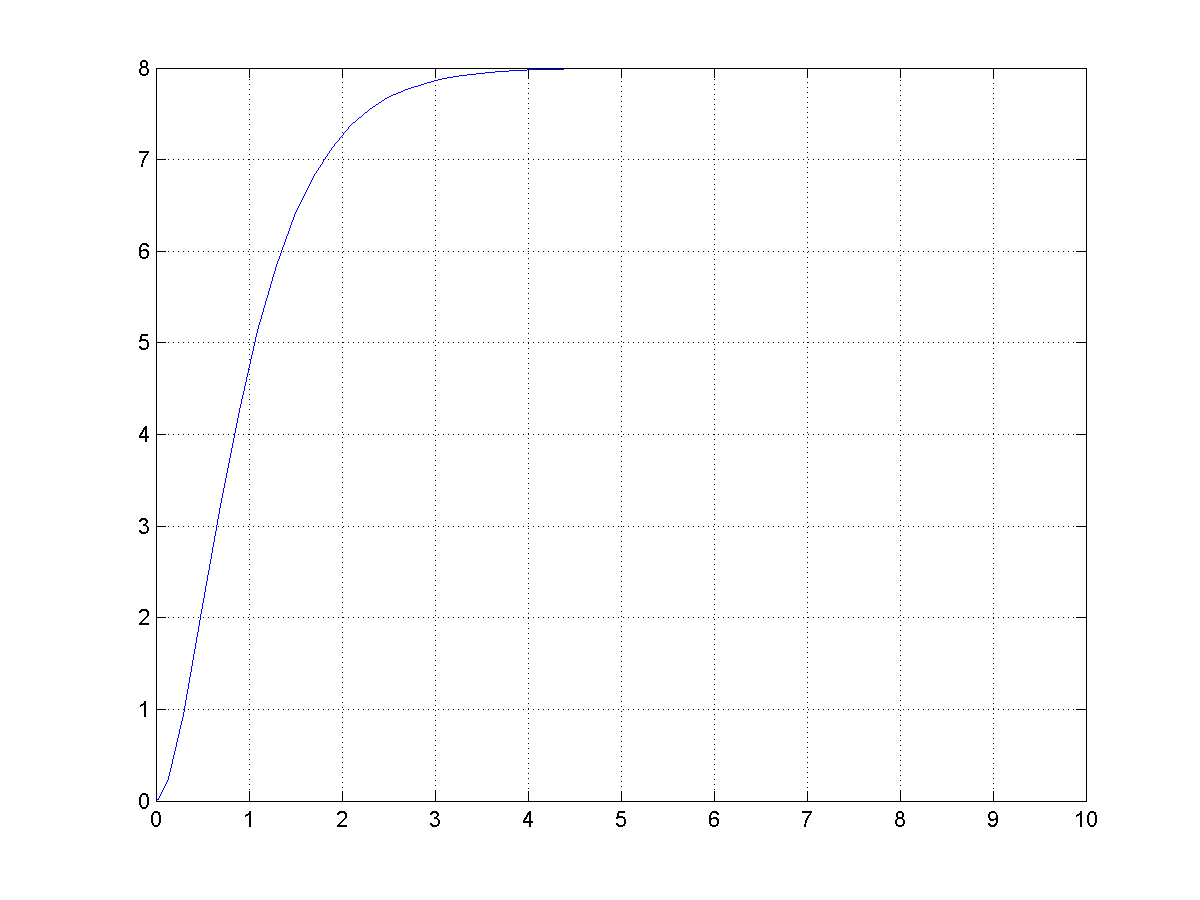
\includegraphics[scale=0.4]{./pictures/i_w2_k8_e1.png}
	\caption{Para $w_{n}$=2, k = 8 e $\xi$ = 1}
	\label{fig:i_w2_k8_e1}
\end{figure}
\begin{figure}[h]
\centering
	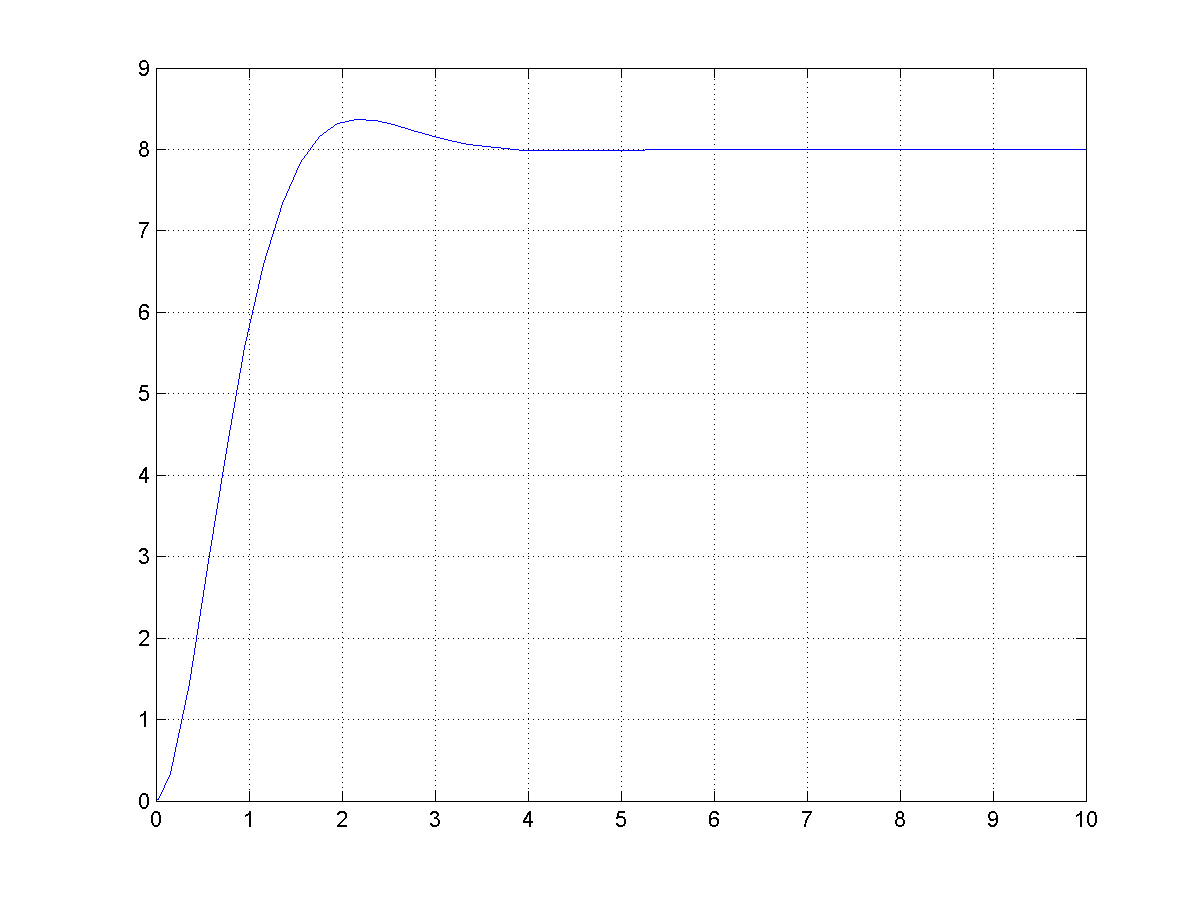
\includegraphics[scale=0.4]{./pictures/i_w2_k8_e07.png}
	\caption{Para $w_{n}$=2, k = 8 e $\xi$ = 0.7}
	\label{fig:i_w2_k8_e07}
\end{figure}
\begin{figure}[h]
\centering
	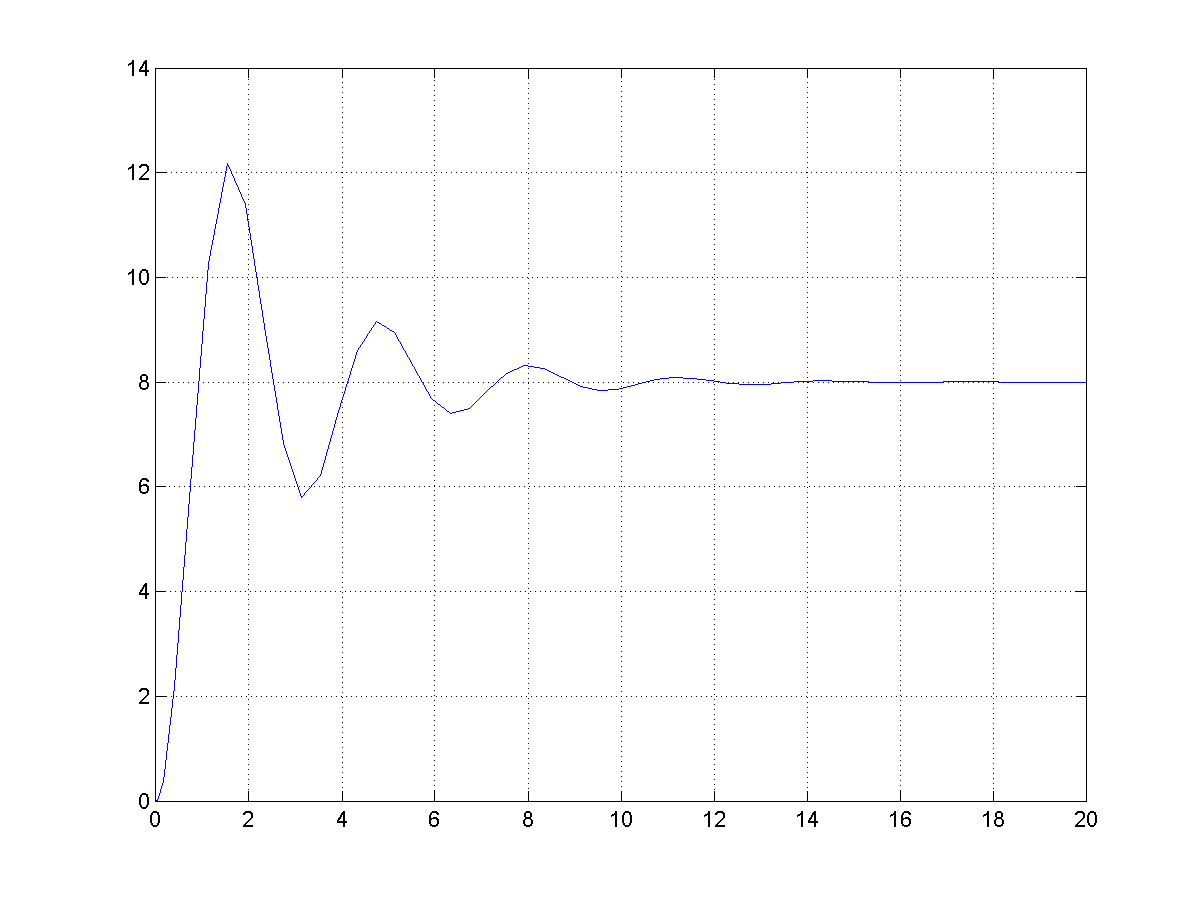
\includegraphics[scale=0.4]{./pictures/i_w2_k8_e02.png}
	\caption{Para $w_{n}$=2, k = 8 e $\xi$ = 0.2}
	\label{fig:i_w2_k8_e02}
\end{figure}
\begin{figure}[h]
\centering
	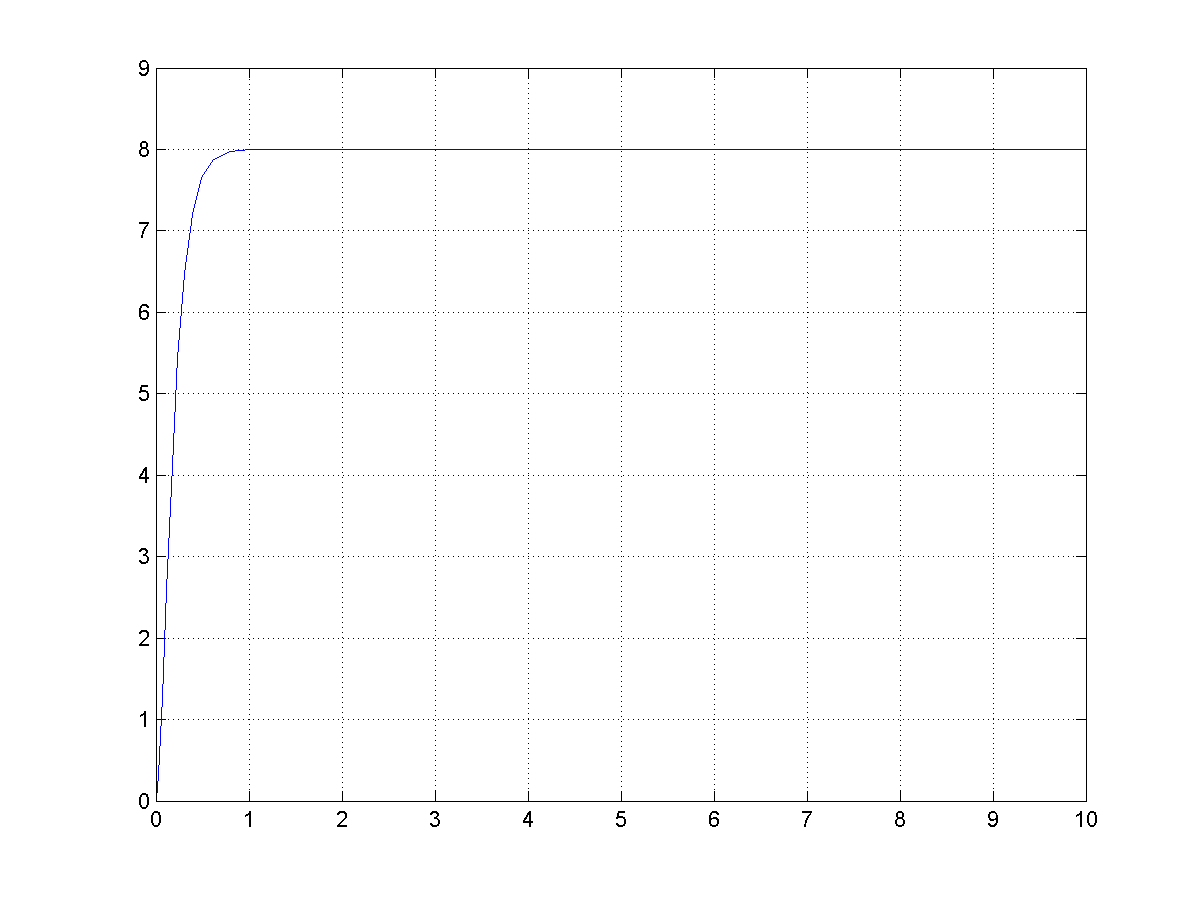
\includegraphics[scale=0.4]{./pictures/ii_w10_k8_e1.png}
	\caption{Para $w_{n}$=10, k = 8 e $\xi$ = 1}
	\label{fig:ii_w10_k8_e1}
\end{figure}
\begin{figure}[h]
\centering
	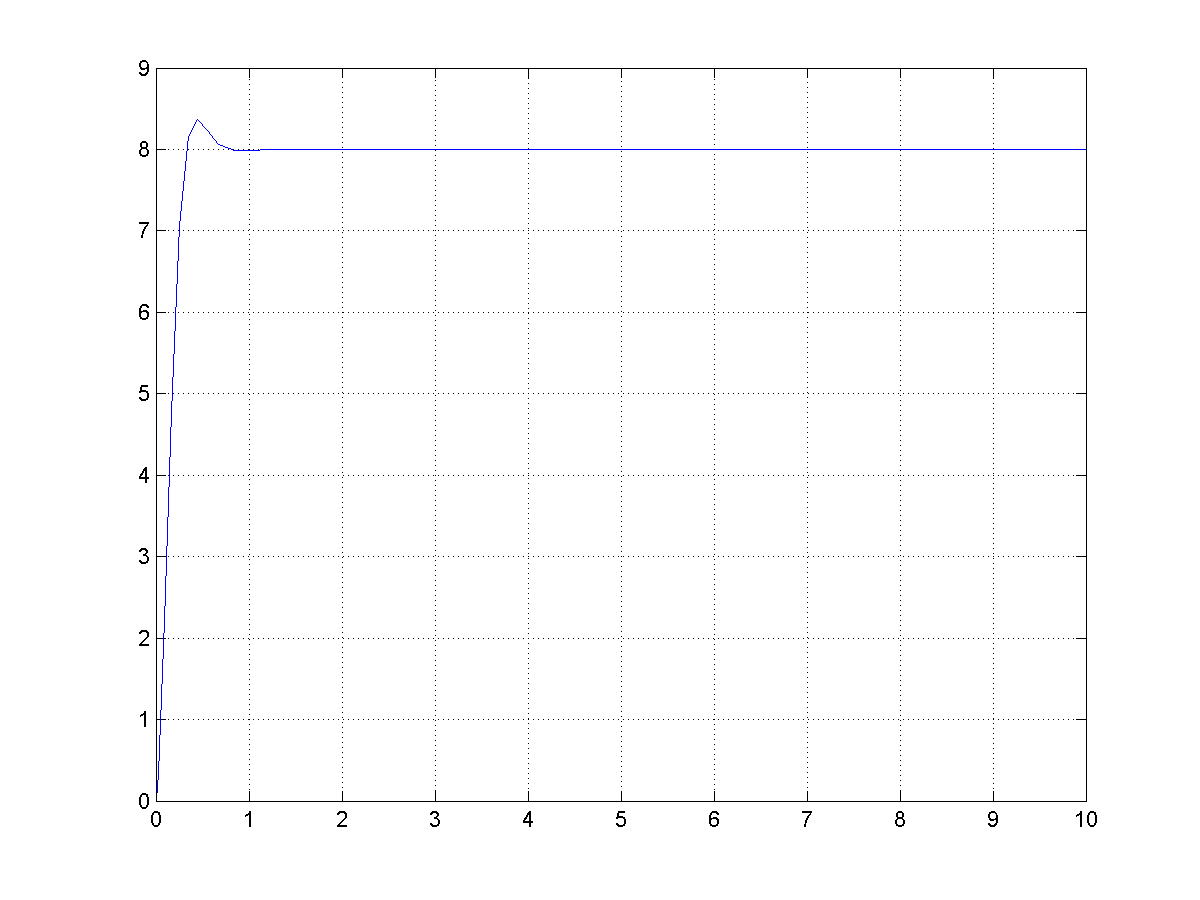
\includegraphics[scale=0.4]{./pictures/ii_w10_k8_e07.png}
	\caption{Para $w_{n}$=10, k = 8 e $\xi$ = 0.7}
	\label{fig:ii_w10_k8_e07}
\end{figure}
\begin{figure}[h]
\centering
	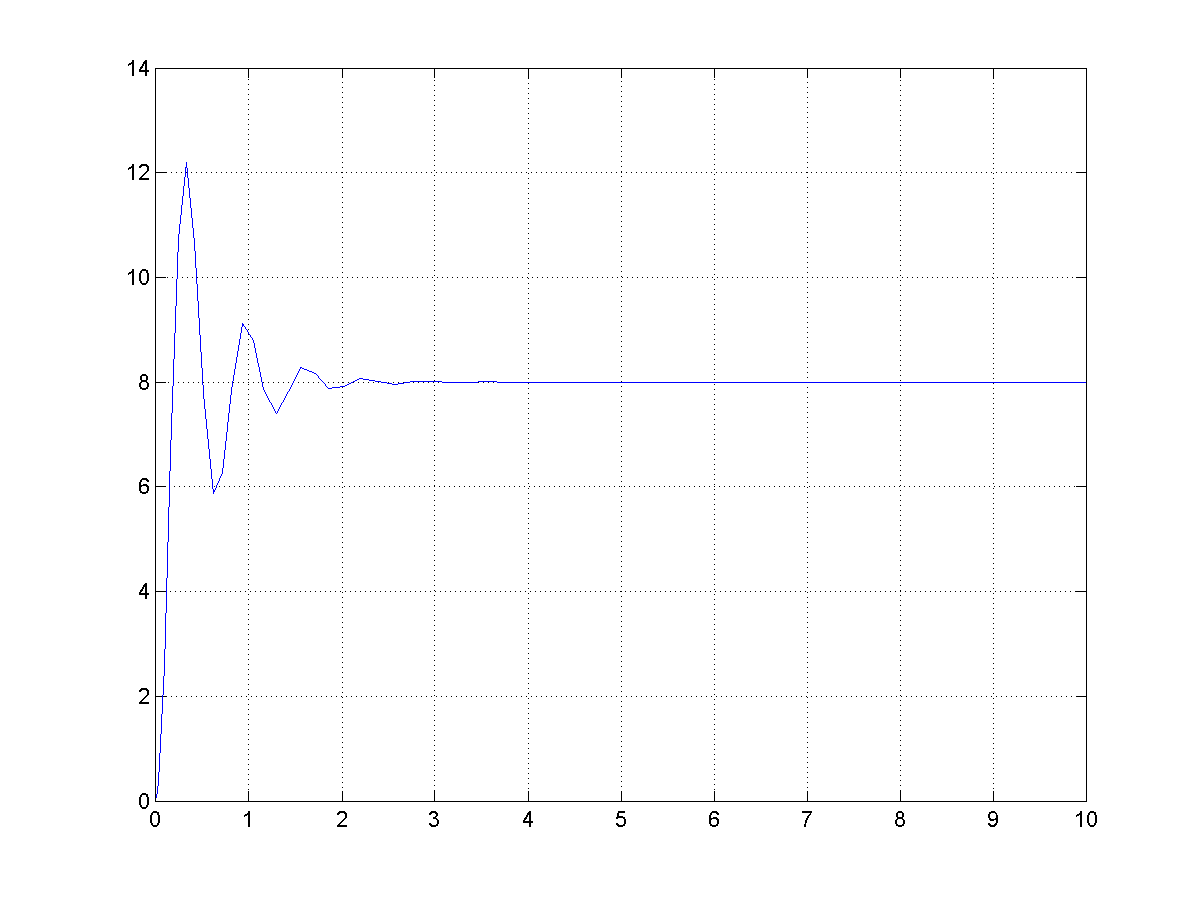
\includegraphics[scale=0.4]{./pictures/ii_w10_k8_e02.png}
	\caption{Para $w_{n}$=10, k = 8 e $\xi$ = 0.2}
	\label{fig:ii_w10_k8_e02}
\end{figure}

\end{document}